\subsection{Model overview}
To model the metabolic the interaction of multiple species populations, each individual was represented as an agent on a grid environment (Figure \hyperref[fig:bacarena]{\ref{fig:bacarena}}).
\begin{figure}[h!]\centering
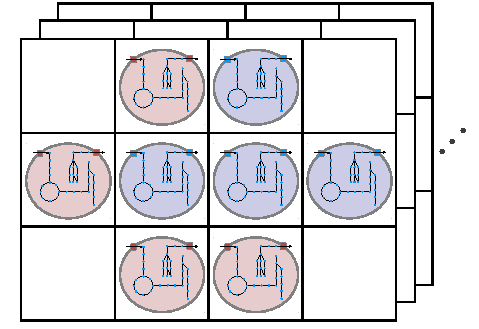
\includegraphics[scale=1.4]{method_chart_BacArena.pdf}
\caption[Overview BacArena]{Overview of the grid environment with two different bacterial agent types (species) in red and blue. Each substrates has its own grid representation.}
\label{fig:bacarena}
\end{figure}
The grid environment was composed of different metabolite concentrations. Furthermore, the species type was recorded for each agent to call the respective genome-wide metabolic reconstruction in every iteration (Algorithm \hyperref[alg:mainloop]{\ref{alg:mainloop}}). The constraints for the subsequent fba were set according to the current metabolite concentrations of the grid cell, where the respective agent was located.
\begin{algorithm}
\caption{Main model iterations called by \texttt{diffbac.R} with different functions applied to bacterial agents and metabolite.}
\SetAlgoLined
\For{number of iterations}{
  \emph{diffusion}()\;
  \For{number of bacteria}{
    \emph{fba}()\;
    \emph{movement}()\;
    \emph{growth}()\;
  }
}
\label{alg:mainloop}
\end{algorithm}
The solution of the fba was used to adjust the biomass of each agent and to modify the metabolite concentrations according to the produced products and consumed substrates. 
This uptake and output of metabolites constituted the exchange with the virtual environment.
A diffusion model was applied to spread the metabolite concentrations over the grid environment and a movement function allowed the random dispersal of each bacterial agent.

A central theme of \texttt{BacArena} was the modularity of each function and metabolic model to allow the extension and replacement of certain parts of the framework. Furthermore, the modularity also enables the inclusion of any desired amount of microbial species. In the following sections the modules of \texttt{BacArena} will be regarded more closely. 

\subsection{Representation}
% -> this should be part of the discussion:
%Implementation began in \textit{netlogo}, which is a simple and wide-used agent based modeling framework.\cite{Wilensky1999}
%For statistical analysis the powerful \textit{R} language was our choice. 
%There exists joint package for interaction of \textit{R} and netlogo (e.g.: \cite{JanThiele2010}), but above all speed limitations led us looking for other possibilities.
%In \textit{R} there exists packages to do agent based modeling e.g. \textit{simecol}, which is an ecological framework with differential equation based approach, too. \cite{Petzoldt2007}.
%But again we could retain performance improvement by simply implementing it ourselves directly in \textit{R}.
The main parts of the framework were implemented in the programming language \texttt{R} ( *). Additionally, certain parts were implemented in \texttt{C++} and integrated in \texttt{R} with the package \texttt{Rcpp} ( *).

\subsubsection{Environment \& Grid}
Agents in \texttt{BacArena} were assigned to specific two-dimensional $n \times m$ grid positions $i, j \in \mathbb{N}$ and a type variable indicating the species. The grid is a discretization of space and could be imagined as a chess board, where the agents can move like chess pieces. 
One single part of the grid is called \textit{cell} with no biological meaning.

For each grid positions certain metabolite concentrations were also recorded and stored in a separate matrix. For each metabolite a own matrix was constructed (Figure \hyperref[fig:bacarena]{\ref{fig:bacarena}}). The bacterial agents could interact with this environment by the consumption and production of metabolite concentrations.

Regarding the grid environment continuous, boundary conditions were chosen, i.e. the rectangle grid is forming the surface of a torus/donut (horn-torus in the case of a square grid).

\subsubsection{Bacteria}
Bacterial populations were represented as a matrix, which had four columns and rows according to the current number of agents on the grid. The first two columns contained the discrete positions of the agents on the grid. The third column indicated the species type of the respective agent. The fourth column stored the current biomass value of the bacteria.

For certain bacterial species, published genome-wide metabolic reconstruction were used as a representation of the individual metabolism by performing flux balance analysis. In the present study the \textit{SBML} models for \emph{Escherichia coli} ( *), \emph{Methanosarcina barkeri} ( *) and \emph{Clostridium beijerinckii} ( *) were used. For each model the metabolites of the published artificial minimal medium (except the respective essential carbon and electron sources) were set to concentrations \emph{ad libitum}. The biomass function for subsequent fba was adopted from the respective \textit{SBML} models. 

According to experimental studies the metabolite fluxes as well as the growth (GAM) and non growth associated maintenance (NGAM) of the models were set to biologically relevant constraints. Those adjusted flux constraints for each model and the respective reference can be found in Table \hyperref[ab:const]{\ref{tab:const}}.

\begin{table}[h!]\centering\footnotesize
\caption{Flux constraints as well as the growth (GAM) and non growth associated maintenance (NGAM) set for each model according to the respective reference. Values are given in $\frac{\mathrm{mmol}}{\mathrm{h}}$.}
\begin{tabular}{lllll}
\toprule
 & \emph{E. coli} & \emph{M. barkeri} & \emph{C. beijerinckii} & Reference\\
\midrule
%\multicolumn{4}{l}{\textbf{Uptake:}}\\
NGAM & 8.39 & 1.75 & 8.5 & ( *)\\
GAM & 59.81 & 30 & 40 & \\
Glucose & 11 & $-$ & 9.39 &\\
Oxygen & 18.2 & $-$ & $-$ &\\
Succinate & 16 & $-$ & $-$ &\\
Methanol & $-$ & 16 & $-$ &\\
Hydrogen & $-$ & 41 & $-$ &\\
Pyruvate & $-$ & 5 & $-$ &\\
Acetate & $-$ & 8 & 3.41 &\\
%\multicolumn{4}{l}{\textbf{Growth:}}\\
\bottomrule 
\end{tabular} 
\label{tab:const}
\end{table}

In each iteration in \texttt{diffbac.R} (Algorithm \hyperref[alg:mainloop]{\ref{alg:mainloop}}), rows were deleted and included according to the growth function (see below). The grid positions were updated according to the movement function and the solution of the fba was added to the current biomass value for each agent.

\subsubsection{Substrate}
Metabolite concentrations were represented as matrices $m_s \in \mathbb{R}^{n \times m}$ for all substrates $s$. According to the requirements of the used Algorithm \hyperref[alg:mainloop]{\ref{alg:mainloop}}genome-wide metabolic models certain metabolites were selected. In the present study these metabolites were: acetate, aketoglutarate, carbon dioxide, ethanol, formate, fumarate, glucose, water, proton, lactate, oxygen, phosphate, pyruvate, succinate, hydrogen, methanol, methane, acetone, butyrate and butanol.
This list can be extended easily by adding another substrate matrix of an arbitrary metabolite with the definition of additional exchange reactions.

According to the simulations of diverse metabolic phenotypes, the matrices of certain metabolites were initialized with a concentration of 70\,mmol per grid cell, whereas the remaining metabolites were initialized with 0\,mmol. 

\subsection{Interactions as rules}
The different representations were closely integrated with each other using rules, which acted on the level of each individual.

\subsubsection{Movement}
To allow the dispersion of the microbial populations, a movement model was implemented (Algorithm \hyperref[alg:move]{\ref{alg:move}}). 
\begin{algorithm}
\caption{Movement of bacterial agents in the von Neumann neighbourhood with $i$ and $j$ as the current positions on the grid.}
\SetAlgoLined
$a \leftarrow i+random(1,-1)$\;
$b \leftarrow j+random(1,-1)$\;
\For{number of bacteria}{
	\uIf{$($a,b$)$ $\in$ bacteria positions}{do not move}
    \Else{$i \leftarrow a$\;
    $j \leftarrow b$\;}
}
\label{alg:move}
\end{algorithm}
Here, each individual agent chooses a random position in the von Neumann neighbourhood, if this cell is not occupied by another microbe. The current two-dimensional grid position is then overwritten with the position of the neighbour. In case the position is located on the boundaries of the grid, the cell on the opposite side of the grid is chosen as a neighbour.
\subsubsection{Diffusion}
For the diffusion of the different metabolites a naive diffusion model was implemented (Algorithm \hyperref[alg:diff]{\ref{alg:diff}}).
%In agent based modeling there are two different rules for updating:
%A Synchronous mode updates all cells simultanously, i.e. local changes are stored in a temporary copy and only after computation of all cells this changes will be efficacious.
%Contrary to this, in a asynchronous mode changes will be made immediately (\cite{Matthies2002} p. 92).\\
%Implementing a simple, naive diffusion model, which interchanges states between neighboured cells, asynchronous updating with randomly choosen cells is preferred because i) synchronouse updating violates conservation laws and ii) nonrandomly asynchronousy is causing a biased diffusion direction \cite{Bandman1999}.
%Further work could be done by implementing more sofisticated diffusion models like block-rotation \cite{Bandman1999} or the discrete diffusion model by Grajdeanu \cite{Grajdeanu2007}.
\begin{algorithm}
  \caption{Diffusion implemented in c++ and included in R using Rcpp \cite{dirk}}
  \SetAlgoLined
  \For{all substrates s}{
    $l \leftarrow 0$\;
    $n \leftarrow$ rows\;
    $m \leftarrow$ columns\;
    \While{$l++ < n \cdot m$}{
      $i \leftarrow random(1,n)$\;
      $j \leftarrow random(1,m)$\;
      $\min$ $\leftarrow$ random local minimum in neighbourhood of cell $i,j$\;
      $m \leftarrow (s(\min_i, \min_j)+s(i,j))/2$\;
      $s(i,j) \leftarrow m$\;
      $s(\min_i, \min_j) \leftarrow m$\;
    }
  }
  \label{alg:diff}
\end{algorithm}
In this strategy, the states of randomly chosen neighbouring cells is interchanged with asynchronous updates. The interchange is implemented by replacing the individual values with the concentration mean of the selected cells.
\subsubsection{Flux balance analysis}
We used fba to represent the metabolic requirements of each microbe in the grid environment.
As described in chapter \ref{cobra} fba determines a flux vector for all reactions by maximizing (in our case) the biomass function.
To solve this optimization problem we used \textit{lpsolve} \cite{lpsolve}, which is available as the \textit{R} package \cite{Rlpsolve}.
The package \textit{lpsolve} is a mixed integer linear programming solver, which is ,,based on the revised simplex method and the branch-and-bound method for integers''\cite{lpsolvedocu}.\\
The respective species specific \textit{SBML} model was loaded for each organism located on the grid (Algorithm \hyperref[alg:mainloop]{\ref{alg:mainloop}}).
In the subsequent fba, several constrains were applied:
\begin{enumerate}
  \item Lower bound of irreversible reaction fluxes is set to $0$
  \item All internal metabolites were assumed to be in flux equilibrium, i.e. $S\cdot v=0$.
  \item Available substrate concentrations control the flux of all exchange reactions (lower bound were set to metabolite concentrations)
  \item Certain empirically validated flux boundaries (Table \hyperref[tab:const]{\ref{tab:const}}) limits exchange reactions even further.
\end{enumerate}
Linear optimization delivers a steady state flux vector $v$, which maximizes the used biomass function. Furthermore, the fluxes were multiplied with the current biomass (accumulated growth) of each microbial agent, to represent the unit of $v$ as $[\frac{\mathrm{mmol}}{\mathrm{g_{DW} \cdot \mathrm{h}}}]$ (higher biomass per dryweight $\sim$ higher fluxes).

The solution flux vector of the fba optimization was taken to redefine the metabolite concentrations on the grid by simple arithmetic operations. Here, all uptake exchange reactions lower the available substrate concentrations in each time step (1\;h) by subtracting the present concentrations with the concentrations taken by the microbe. Conversely, the providing exchange reactions raise the product concentrations in each time step (1\;h) by adding the concentrations produced by the microbe to the present concentrations.

To represent the biomass the individually determined growth rates $[\frac{\mathrm{mmol}}{\mathrm{g_{DW} \cdot \mathrm{h}}}]$, defined by the flux through the biomass function according to the available substrates, were added to the existing biomass of each microbe. Therefore, the biomass accumulated in each time step (1\;h).

\subsubsection{Growth}
Microbial growth was considered as the output of the fba-optimized biomass function. In case the fba did not find a solution, we considered a starvation phase, in which biomass was consumed. 
To produce population dynamics, two different processes were part of the model:
\begin{enumerate}
	\item \textbf{Duplication}: Biomass accumulation allows the microbial reproduction (duplication).
	\item \textbf{Death}: Starvation consumes the available biomass and leads to ultimate cell death.
\end{enumerate}
\paragraph{Duplication}
The growth (GAM) and non growth associated maintenance (NGAM) was adopted from the literature individual microbe species (Table \hyperref[tab:const]{\ref{tab:const}}). NGAM, accounts for the obligatory ,,housekeeping'' energy consumption of each cell, whereas GAM represents the energy consumption necessary for replication. 

In \texttt{BacArena} all microbe agents start with a initial biomass of $1$ symbolizing an intact cell. If the accumulated biomass in the growth model reaches the double amount of the initial biomass, duplication was enabled. The daughter cell was randomly placed in the direct neighbourhood of the parent, similarly to Algorithm \hyperref[alg:move]{\ref{alg:move}}. In this process the current biomass was equally divided between daughter and parent cell. If the chosen grid position is occupied by another microbe the daughter cell was removed (death).
\paragraph{Death}
Flux balance analysis considers a fixed NGAM flux and growth depending GAM part of the biomass function.
Under starving conditions, where no fluxes according to fba calculations can be found, we considered the current biomass as a reservoir, from which the cell can ,,feed'' on. The biomass was subsequently reduced with
\[
  \textrm{biomass}_{\,t+1} = -\frac{\textrm{NGAM}}{\textrm{GAM}}\cdot \textrm{biomass}_{\,t}+\textrm{biomass}_{\,t}
\]
which is dependent on the adopted NGAM and GAM values of each individual \textit{SBML} model (Table \hyperref[tab:const]{\ref{tab:const}}). The microbe agents were removed from the grid environment (death), if their current biomass was lower than the arbitrary threshold of 0.